\section{Introducción}
En este capítulo, se entrenarán modelos de texto utilizando redes neuronales recurrentes con LSTM. El objetivo será generar sucesiones de texto que parezcan reales. Para hacer esto, se procesarán y entrenarán los modelos con diferentes bases de texto y después se generarán las sucesiones de la siguiente manera: se sampleará la distribución del modelo y después la predicción se utilizará como dato de entrada para el siguiente paso. En otras palabras, como explica (Graves, 2013), el modelo trata a sus invenciones como si fueran reales, de la misma manera que lo hace una persona cuando sueña. Para decidir los hiperparámetros de los modelos se utilizó como base el artículo mencionado de Alex Graves, así como el artículo $``$The Unreasonable Effectiveness of Recurrent Neural Networks$"$ escrito por Andrej Karpathy, estudiante de doctorado en aprendizaje profundo en Stanford.
\cite{DBLP:journals/corr/Graves13}
\cite{unreasonable}

\vspace{1em}

Se utilizarán 3 bases de texto diferentes y se compararán los resultados obtenidos. El primer texto que se utilizará será el libro Rayuela de Julio Cortazar, el segundo, será La Biblia en inglés y por último se utilizará datos para generar muestras de Wikipedia.

\vspace{1em}

Aunque generalmente los modelos de lenguaje se hacen a nivel palabra, en este trabajo se harán a nivel caracter. Esto se debe a varias razones. Por un lado, si el análisis se hace a nivel palabra, como el número de palabras es muy grande (a veces mayor a 100,000 incluyendo diferentes conjugaciones, nombres propios, etc.), el número de clases y parámetros es demasiado grande y eso aumenta el costo computacional. Por otro lado, predecir un caracter a la vez es más interesante desde el punto de vista de generación de sucesiones porque permite al modelo crear nuevas palabras. Por lo tanto, siguiendo el trabajo de (Graves, 2013), se predicirá con la granularidad más fina, nivel caracter, para maximizar la flexibilidad del modelo.
\cite{DBLP:journals/corr/Graves13}

\section{Descripción de las bases de datos}

A continuación se describirá cada base de datos y los modelos que se utilizarón para cada análisis. Los bases de datos y los modelos utilizados se pueden encontrar en el siguiente repositorio: https://github.com/GeorBelanger

\subsection{Rayuela}
Este libro de Julio Cortazar escrito en París y publicado en 1963 es una de las obras centrales del boom latinoamericano. En ella, Cortazar invita al lector a leer sus 155 capitulos en el orden que desee, por lo que se le suele llamar una $``$antinovela$"$ y esto hace que tenga una estructura interesante para generar nuevas sucesiones de ella.
Esta base de datos se obtuvo de la página del Instituto Latinoamericano de la Comunicación Educativa (ILCE). Esta base tiene 972,231 caracteres y los conjuntos de validación y prueba tienen cada uno 100,000 caracteres.
\cite{rayuela}
\cite{cortazar}


\subsection{La Biblia}
La Biblia es uno de los libros más leídos y más famosos de la historia. Este texto está en inglés y se obtuvo de NLTK ($``$Natural Language Toolkit$"$), una plataforma dedicada a trabajar con datos de lenguaje humano. Esta base tiene 4,123,223 caracteres y los conjuntos de validación y prueba tienen cada uno 500,000 caracteres.
\cite{nltk}

\subsection{Concurso Hutter}
Finalmente, siguiendo el trabajo de (Graves, 2013), se considero el conjunto de datos del concurso $``$Hutter$"$. Esta base de datos contiene los primeros 100 millones de bytes de la página de Wikipedia en inglés. El archivo no solo incluye los datos comprimidos sino también el código para implementar el algoritmo de compresión. Además de contener muchas palabras del diccionario, la base de datos contiene muchas sucesiones de caracteres que normalmente no se usarían como por ejemplo etiquetas XML para definir los meta-datos, direcciones de páginas de internet y markup para formatear los datos (encabezados, listas, etc.). Esta base de datos contiene 82,551,973 caracteres y los conjuntos de validación y prueba tienen cada uno 1,000,000 de caracteres.
\cite{DBLP:journals/corr/Graves13}


\section{Resultados}
A continuación se mostrarán los resultados para cada uno de los modelos.

\subsection{Modelo Rayuela}
Para esta base de datos se utilizó una red neuronal recurrente con unidades LSTM. Este modelo empleó una tasa de aprendizaje inicial de 0.03, a Adam como algoritmo de optimización, un recorte de gradiente con cota de 1, el tamaño de las batches fue de 100 y las sucesiones que se analizaron tuvieron una longitud de 50 caracteres. En todos los modelos se utilizó detención temprana.

\vspace{1em}

En primer lugar se corrió una red neuronal con 1 capa oculta con 100 unidades LSTM. Después de cada época, es decir, cada corrida de entrenamiento por todos los datos, se evaluó el error de validación y se generaron sucesiones de 500 caracteres de longitud. En la figura 4.1 se pueden ver las primeras dos épocas. En las generaciones de texto, se puede ver que en la primera época el modelo empieza a aprender a separar las palabras con espacios de tal forma que tengan una dimensión razonable (2-8 caracteres). Después de la segunda época se puede ver que el modelo ya ha aprendido algunas palabras básicas del español: como, sobren, de, la, cosa, pan, etc. Todavía está un poco lejos el modelo generar sucesiones en español. 

\begin{figure}[h]
\begin{center}
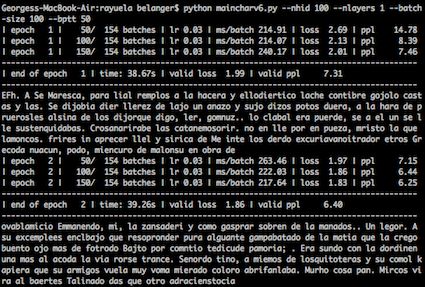
\includegraphics{./imag/ray11.png}
\end{center}
\caption{}
\end{figure}


En la figura 4.2, se puede ver el mismo modelo en las últimas dos iteraciones y la evaluación del error de prueba. El modelo ahora ya genera palabras más complejas en español y se puede ver que incluso ha aprendido el nombre del personaje principal de la obra: Oliveira. No obstante, el modelo sigue lejos del desempeño esperado. Se puede ver que el error de prueba fue menor que el error de validación, por lo que no se está sobreajustando. Se intentará utilizar modelos con más parámetros para mejorar el desempeño.

\begin{figure}[h]
\begin{center}
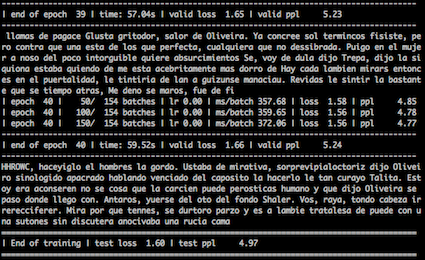
\includegraphics{./imag/ray12.png}
\end{center}
\caption{}
\end{figure}

\vspace{1em}

Para mejorar la calidad de las sucesiones, se aumentó la capacidad del modelo y luego se utilizó regularización para evitar sobreajustar. Se optó por un modelo de dos capas ocultas y 500 unidades ocultas y se utilizó dropout después de cada capa oculta. El error de validación con detención temprana resultó ser 1.64 y el error de prueba 1.60, por lo que parece ser que todavía no se está sobreajustando. A continuación se muestra una sucesión generada con este modelo. 

\vspace{1em}

$``$A Pola como un estecho una salia esos fodido de cosas un dido... A nadie que a los caleungo de Oliveira. A oble Mont reputados que mi cientos dijo Tenrico de que vez. Mane, un estobadon, la busto estus fudente. Hecidos ejemposo dijo Talita y ventan En sido nos parata -laguo opirosa. Un que rearder. Remuodo esperana como Mato de tilonis, que fuera realmente Arren con gris, y asmiento el piersko quina si Se la mas hucha hasta los acorrino un bubio. Es salibles en pasa$"$

\vspace{1em}

Se puede ver que este modelo genera muchas palabras en español o con estructura del español y las frases hacen más sentido que en el modelo anterior. Una de las razones que pueden estar frenando un mejor desempeño es lo pequeño de la base de datos. En el siguiente experimento se utilizará una base de datos 4 veces más grande y se compararán los resultados.


\subsection{Modelo Biblia}
Para esta base de datos se utilizó el mismo modelo que con los datos de Rayuela. Es decir, una red neuronal recurrente con unidades LSTM, una tasa de aprendizaje inicial de 0.03, a Adam como algoritmo de optimización, un recorte de gradiente con cota de 1, el tamaño de las batches fue de 100 y las sucesiones que se analizaron tuvieron una longitud de 50 caracteres. En todos los modelos se utilizó detención temprana y dropout como regularización.

\vspace{1em}

Esta base de datos es bastante más grande que la de Rayuela, por lo que el tiempo de entrenamiento aumenta también. Como primer modelo se utilizará 1 capa oculta con 100 unidades LSTM y a dropout como algoritmo de regularización después de cada capa oculta. Este modelo converge rápidamente y entrega mejores resultados que los experimentos con Rayuela. A continuación se verá una sucesión que se generó con este modelo.

\vspace{1em}

$``$Sheb, of kings your childres. The midst that and thou fall they say a rain stangues, with thou and seadwe, that that he for the leses, I mave knet and is somongel; unto him, besought this shoot. And the inholire she blood savids ye also tendenshaln my fompest; and the tritiel merle who einssyres as all usterly not which all man out over, even the word givity at he be it awonk whom even out whous him$"$

\vspace{1em}

Este modelo ya produce casi todas las palabras en inglés o a veces palabras que no existen, pero que tienen una estructura similar a la del idioma inglés. A continuación, se utilizó un modelo con una mayor capacidad: 1 capa oculta con 500 unidades LSTM.

\vspace{1em}

El modelo con 1 capa oculta y 500 unidades LSTM convergió en 6 épocas y entregó muy buenos resultados. El error de validación fue de 1.17 y el de prueba de 1.21, y a continuación se puede ver una sucesión que se generó con este modelo:

\vspace{1em}

$``$But Jeah said ut into the LORD God and these day of thine of that dwelt my God because of the priests swalling is also not gate of thiel, have spirit if us weed, but with them put her's lasting, and their judgest covered their tarrim to them, and please God which connembrory. But the first before him, and in my servant and sinate;$"$

\vspace{1em}

Este modelo ya escribe inglés bastante bien y algunas partes de las frases empiezan a tener sentido. La tabla 4.1 contiene los tiempos de entrenamiento y los errores de validación para cada época. Se puede ver que el valor de validación desciende hasta la sexta época y después empieza a aumentar. Debido a que se está utilizando detención temprana, el modelo de que se tenía en ese momento es con el que se evalua el error de prueba.

\vspace{1em}



\begin{table}[htbp]
\begin{center}
\begin{tabular}{&l&l&l&}
\hline
Final de la época   1 & tiempo: 983.04s & error valid  1.62 & ppl valid     5.07
\\ \hline
Final de la época   2 & tiempo: 1018.08s & error valid  1.39 & ppl valid     4.02
\\ \hline
Final de la época   3 & tiempo: 958.67s & error valid  1.32 & ppl valid     3.76
\\ \hline
Final de la época   4 & tiempo: 972.85s & error valid  1.26 & ppl valid     3.52
\\ \hline
Final de la época   5 & tiempo: 984.16s & error valid  1.19 & ppl valid     3.28
\\ \hline
Final de la época   6 & tiempo: 1084.37s & error valid  1.17 & ppl valid     3.23
\\ \hline
Final de la época   7 & tiempo: 984.27s & error valid  1.17 & ppl valid     3.24
\\ \hline
Final de la época   8 & tiempo: 1065.81s & error valid  1.18 & ppl valid     3.25
\\ \hline
Final de la época   9 & tiempo: 2404.71s & error valid  1.23 & ppl valid     3.41
\\ \hline
Final de la época  10 & tiempo: 4644.00s & error valid  1.41 & ppl valid     4.09
\\ \hline
Final del entrenamiento & & error de prueba  1.21 & ppl prueba    3.34
\end{tabular}
\caption{Resultados del entrenamiento del modelo}
\label{Entrenamiento del modelo}
\end{center}
\end{table}

La tabla 4.2 contiene generaciones de sucesiones para las 6 primeras épocas, momento en el que el modelo alcanza su mejor desempeño. Se puede ver como las sucesiones van mejorando conforme el modelo disminuye su error de validación.

\begin{table}[htbp]
\begin{center}
\begin{tabular}{&}
\hline
qum noth, I wald ame is he wils. Befemod; whe vied that \\ 
the camem by in the entick not will the draad, fore priecy of were 
\\ \hline
ual to gindes ye depers will come cannted of his natering\\ 
whines I will s happerats. But God of his couse a scaight against 
\\ \hline

and ye there servens trought the land of a bread, when me\\
As come Behold, neither Ham, all not done offer on his dead wrire 
\\ \hline

e hear he lift firdness bour mine pon, and Shew as one \\ 
uncity, and Gad what unto commandmenteth in the intip Joht it to 
\\ \hline

e to Hali, saying, Gameth, are dwelling place the irmine\\
of him. For in truck in thy Surely, and all all Israel, We doth 
\\ \hline

rives seakand king's bediefliseth, and I sike them being\\
even them fear in Ghist have my people had we shall see the mess 
\\ \hline
\end{tabular}
\caption{Generacion de sucesiones para cada época}
\label{Generaciones}
\end{center}
\end{table}


Se obtendran más sucesiones de este modelo al hacer variar la temperatura de la softmax de salida. La temperatura es simplemente un número por el que se divide el vector de salida antes de aplicarle la función softmax. Por lo tanto, al disminuir la temperatura de 1 a 0.1, aumenta la confianza de las predicciones de la red, pero también será más conservadora. A continuación se muestra una muestra utilizando 0.1 como temperatura.
\cite{unreasonable}

\vspace{1em}

$``$uhus thine sin to the servone of the son of King is shall the morning and the same of the son of King and the son of Assyria the son of King is shall the servont to the same the same that said unto them, The LORD shalt the same the same of the same the same the same that he said unto them, The LORD said unto them, $"$

\vspace{1em}

Se puede ver que como el modelo es más conservador, entrega sucesiones que son más probables que estén escritas en la Biblia, pero, al mismo tiempo, esto hace que se generen ciclos de frases que aparecen mucho en el conjunto de entrenamiento como por ejemplo $``$the son of King$"$. Este problema se puede solucionar elevando un poco la temperatura, como se muestra a continuación con una sucesión generada con 0.5 de temperatura.

\vspace{1em}

 $``$And in the house of the LORD in the corner in the mercy of the stones and the children of Israel the prophesy and how will seek a litter is sin. And the mighty of it is a standed me with the things the first the wicked in the sons of Saul the play of the word of the son of Kanah, and at the singer of the morning that have in the word of the LORD and the word of the LORD and the standing of the LORD, and went in the people came out of God.$"$
 
\vspace{1em}

Las palabras ahora son casi todas del idioma inglés y las frases ya empiezan a tener sentido. Al ver estos resultados, se puede ver que el modelo ya genera sucesiones que se aproximan razonablemente al texto analizado. Ahora, se probarán estos modelos con el texto del concurso Hutter, el cual tiene una estructura un poco más complicada que los primeros dos.

\subsection{Modelo Hutter}
Esta base de datos utilizó un modelo muy parecido a los dos anteriores. Es decir, una red neuronal recurrente con unidades LSTM, una tasa de aprendizaje inicial de 0.03, a Adam como algoritmo de optimización, un recorte de gradiente con cota de 1. Para este modelo, debido a sus mayores dimensiones, el tamaño de las batches que se utilizaron fue de 1000 y las sucesiones que se analizaron tuvieron una longitud de 50 caracteres. En todos los modelos se utilizó detención temprana y dropout como regularización.

\vspace{1em}

Esta base de datos es bastante mayor que las otras dos, por lo que cada época tiene una mayor cantidad de datos. En primer lugar, se empleó un modelo con 1 capa oculta y 100 unidades LSTM. El modelo convergió en 3 épocas. El error de validación al final de la tercera época fue de 1.77 y el de prueba fue de 1.73, por lo que parece ser que no se está sobreajustando. Estos resultados están lejos del desempeño esperado por lo que se probarán modelos con más parámetros. A continuación, en la tabla 4.3, se muestran algunas sucesiones generadas por este modelo. 

\begin{table}[htbp]
\begin{center}
\begin{tabular}{&}
\hline
Shelt be *Arlant tech-th leanve's in [[Emperies Gensrotuc' continonicums \\ Joker]] \&lt;sup\&gt; Wicywarth ISBN]] *[[Ansorsurine Ass anner Highn]]
\\
\\ \hline

Austriality woul mentioned by [[Brath ]] house special [[Whes Cack'' anver \\ prefine datasen]] Wicard.a</text tiems] [[Ajfhs]])
\\ 
\\ \hline

* [http://www.abrithul.lolmarc'' was throrss parer\&lt;br\&gt; pound with \\ inderon be unteendicity and invernity
\\ 
\\ \hline

[[Qumose jurn|[[meltorit]], [[Nature leathers plits]])|hill Effice]] \\ *[[mplet;, Aarc, Strege United WPTR, Afn Husi]]
\\ 
\\ \hline


\end{tabular}
\caption{Sucesiones con primer modelo de Hutter}
\label{sucesiones hutter 1}
\end{center}
\end{table}

Se puede ver en estas sucesiones que el modelo ya esta aprendiendo de los datos a escribir inglés y a abrir y cerrar paréntesis bastante bien. Incluso genera direcciones web imaginarias. Se va a utilizar un modelo con más parámetros para aprender más sobre la base de datos.

\vspace{1em}

El siguiente modelo que se probó utilizó una capa oculta y 500 unidades LSTM ocultas. También se utilizaron batches de tamaño 1000 en esta ocasión. En la tabla 4.4 se muestran los errores de validación y los tiempo de entrenamiento  para las primeras 4 épocas.

\begin{table}[htbp]
\begin{center}
\begin{tabular}{&l&l&l&}
\hline
Final de la época   1 & tiempo: 23473.43s & error valid  1.60 & ppl valid     4.95
\\ \hline
Final de la época   2 & tiempo: 34589.61s & error valid  1.54 & ppl valid     4.68
\\ \hline
Final de la época   3 & tiempo: 31840.15s & error valid  1.49 & ppl valid     4.43
\\ \hline
Final de la época   4 & tiempo: 42349.47s & error valid  1.48 & ppl valid     4.41
\\ \hline
Final del entrenamiento & & error de prueba  1.44 & ppl prueba    4.22
\end{tabular}
\caption{Resultados del entrenamiento del modelo}
\label{Entrenamiento del modelo}
\end{center}
\end{table}


Como se puede ver en la tabla, el error de validación empieza a converger depsués de la época 4. Se puede ver que el tiempo de entrenamiento para cada época ha aumentado a más de 30,000 segundos, es decir, más de 8 horas. Esto se debe en parte al tamaño de la base de datos y al número de parámetros que se tienen que actualizar. En la tabla 4.5, se muestra varios ejemplos de sucesiones generadas con el modelo.


\begin{table}[htbp]
\begin{center}
\begin{tabular}{&}

\\ \hline

[[Image:Sera Jurischoshaavireson in Expexed a name, diversion of Oe \\ Tagtonninans Players #Lemen]] [[Category:Ort Category:Stera de \\ Carregrowing]] {{Heaps such}} [[Category:Horn|General General]]
\\ 
\\ \hline

The [[first sea]] and the glast level major most bally on the gla the \\ antitrone hard, the Thind national Depass or earnenton, entropy and a'' et \\ teams of '''National fargular)
\\ 
\\ \hline

Gallamorboniauist on the did not combinative name ones and physically early \\ \&quot; has \&quot; of the environt, and support as a [[Each chase]] \\ whyrigal later term in thome, each ancient authoring as a particularly subspace
\\ 
\\ \hline


\end{tabular}
\caption{Sucesiones con segundo modelo de Hutter}
\label{sucesiones hutter 1}
\end{center}
\end{table}

Al examinar las sucesiones de la tabla 4.5, se puede ver que el modelo no solo ha aprendido palabras en inglés, sino que también las estructuras de sus frases empiezan a tener sentido y ha aprendido a abrir y cerrar brackets así como otros símbolos como el hashtag # y hacer \&quot. En la tabla 4.6, se analizarán algunas sucesiones al modificar la temperatura a 0.5.

\vspace{1em}




\begin{table}[htbp]
\begin{center}
\begin{tabular}{&}

\\ \hline

\{\{ref\| \| \|\| \|\| \|\- \| \| align=\&quot;left\&quot;\|\| \|\| \|\| \|\| \|\| \|\| \|\| \{\{cite of \\ the stilled on the cannot to the real and about patents and \\ international money of an office
\\ 
\\ \hline

texts= The Death (for the game of world that and the series and working \\ state and in the record leaders controlled as a talk of an international \\ termant on the series in many allowing the same extra the plate, the round \\ and in the process, is particular from the former the particular on the [[spain]]
\\ 
\\ \hline

The [[central war]] and the [[representation]] and [[antiton]], factors and \\ party of the world that entertainment on the attempts to all and exports \\ by the assumes of a tall are projected to the serious are the people
\\ 
\\ \hline


\end{tabular}
\caption{Segundo modelo de Hutter: temperatura 0.5}
\label{sucesiones hutter 1}
\end{center}
\end{table}

En las sucesiones de la tabla 4.6, se puede ver que el modelo ya escribe bastante bien inglés, sabe abrir y cerrar paréntesis y  tienen intuiciones del lenguage markdown que utiliza el documento, como en el primer ejemplo: $``$align=\&quot;left\&quot;$"$. 

\vspace{1em}

Los resultados aquí mostrados están lejos aquellos mostrados por (Graves, 2013). Sin embargo, esto se puede explicar por la capacidad computacional a la que se tiene accesso. Graves, en su artículo, al analizar la base de datos del Premio Hutter, utiliza 7 capas ocultas con 700 unidades LSTM en cada una, un modelo que sería muy dificil y tardado de optimizar utilizando la computadora que se tiene disponible para hacer este trabajo.
\cite{DBLP:journals/corr/Graves13}